\section{Results}

The training and validation history of loss function and accuracy for RoBERTuito is in figure \ref{fig:history}. This model with the hyperparameters from table \ref{table:hyperparameters} obtain a 0.89143 on F1-Score Macro on the test dataset. This value was calculatd with the Kaggle Forum. With a bigger number on epochs, the F1-Score is reduced to 0.82 or 0.80. The learing rate (lr) can be 2x10$^{-5}$, this value can produce same F1-Scores, but if the lr increase or decrease more the F1-Score will be lower. The model was based in this blog \href{https://towardsdatascience.com/how-to-train-bert-aaad00533168}{How to Train BERT}.

\begin{figure}[H]
    \centering
    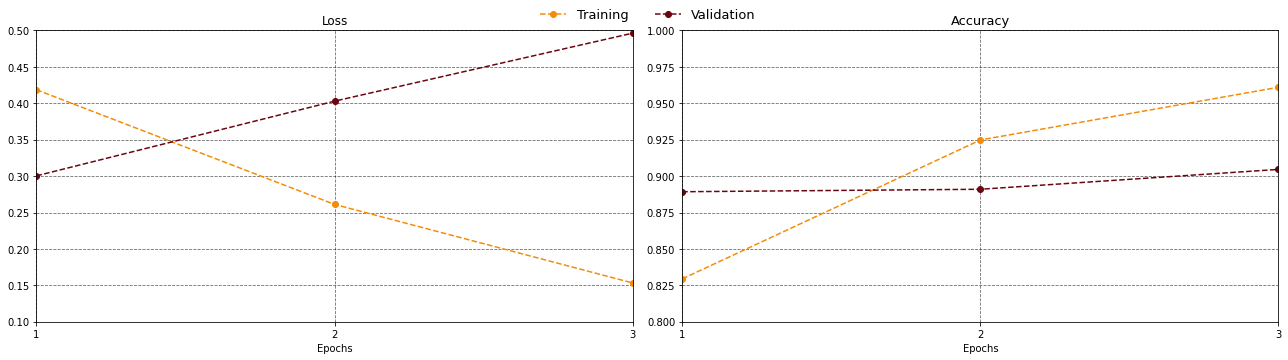
\includegraphics[width=15cm]{Graphics/history.png}
    \caption{Training and validation history of loss function and accuracy.}
    \label{fig:history}
\end{figure}